% -----------Incluir esto en caso necesario para que el capítulo comience siempre en página impar

%\newpage
%\thispagestyle{empty}
%\mbox{}
%---------------------------------------

\chapter{Introducción} 
\label{ch:chapter1}
\setlength{\parindent}{0cm}
\setlength{\parskip}{4mm}

\section{Motivación}\label{Motiv}

Un problema en la actualidad son las aguas contaminadas por agentes de origen biológico, su importancia recae en la perdida de la biodiversidad y en que implican daños perjudiciales en la salud humana dado que las sustancias presentes en el agua pueden ser ingeridas por las especies marítimas que posteriormente son consumidas por los seres humanos.

Un aspecto fundamental sería el detectar y caracterizar la distribución de dicha contaminación. Por ende, tomando en cuenta los avances tecnológicos de los sistemas robóticos de hoy en día, llegándose a considerar incluso como sistemas autónomos y programables capaces de realizar diversas tareas, se propone como objetivo de este proyecto el otorgar la capacidad de detectar y guiar a un conjunto de vehículos dispuestos sobre una superficie marítima hacia zonas de máxima concentración de sustancias toxicas.

Los vehículos han de tener la capacidad de reunir datos del entorno, dicha tarea se realiza al estar dotados de sensores adecuados, emplazados en puntos fijos y de diversos tipos para tomar medidas de nivel de contaminación de modo continúo para posteriormente convertirlos en acciones a través de su efector final.

Un vehículo que engloba todas las características descritas hasta el momento son los USVs \footnote[1]{unmanned surface vehicle} cuyo uso recae en tareas de monitorización de las aguas de manera automático y desasistido.

Además, al tratarse de una tarea que implica cubrir zonas amplias de agua, una manera más eficaz de acometerla es el empleo de multiples USVs que cooperan eficientemente entre ellos para cumplir la labor asignada. Esto conlleva a una necesidad de coordinarlos, en donde, existen diversas formas de hacerlo tal como se puede apreciar en \cite{Otra_Coorporativa}. En este proyecto se va a centrar en \cite{Control_Formacion} basado en la cooperación entre los USVs consiguiendo un sistema descentralizado y robusto.\\

\begin{figure}[htb]
\centering
\includegraphics[width=0.6\textwidth]{figures/USV.eps}
\caption{Ejemplo de USV. Figura obtenida de: \url{https://www.navalnews.com/naval-news/2019/02/eca-group-unveils-inspector-125-unsinkable-usv/}}\label{fig:USV}
\end{figure}

El proceso principal para la detección de los agentes biológicos en aguas contaminadas es la búsqueda de la fuente de contaminación. Por ello el objetivo de este proyecto consiste en ver cómo un conjunto de agentes son capaces de comunicarse entre ellos para detectar el foco de máxima concentración para posteriormente desplazarse hacia él satisfactoriamente.

Consecuentemente, los vehículos han de ser capaces de cumplir dos roles fundamentales, en primer lugar ser capaces de detectar exactamente el punto de origen de máxima concentración y en segundo lugar coordinarse para ejercer el desplazamiento definiendo una forma simétrica concreta. Entre otras palabras, se requiere aplicar al caso un enjambre robótico más concretamente uno de tipo multiagente.

Cabe añadir que el punto de máxima concentración en la superficie sobre la que se desplazan los vehículos se puede definir mediante las curvas de nivel, además su variación se puede suponer que va a estar ligada con la distancia a la que este el centro de la formación con respecto al punto máximo, es decir, la intensidad radiada desde el punto fuente es una señal proporcional al inverso de la distancia al cuadrado.

Asimismo, en cualquier punto de la superficie del agua afectada por los agentes biológicos, el gradiente de la concentración apunta en la dirección de crecimiento de la contaminación y por tanto hacia la fuente. Una forma de llegar al máximo es ir tomando medidas de manera continúa con los sensores acoplados en cada USVs para ir avanzando en función de la dirección marcada por dicho gradiente, en donde si este se anula quiere decir que los vehículos han llegado al punto máximo.

Finalmente, para llevar a cabo el calculo del gradiente se utilizará un grupo de robots que lo estimarán tomando medidas de contaminación en un punto haciendo uso de sus sensores, con estas se podrán guiar hasta el máximo de la concentración.

\section{Estado del arte}\label{Objetives}

La robótica de enjambre se basa en el comportamiento de los organismos sociales, en donde los individuos no han de tener un alto conocimiento para producir un comportamiento colectivo complejo, ni existir un líder que guía al resto para completar un objetivo, como en los bancos de peces, un panal de abejas o una bandada de pájaros.

Hoy en día, conforma un área de investigación muy activa por su versatilidad en diferentes ámbitos, tales como militar o industrial. En contraposición a tener un único robot realizando una labor compleja se tienen varios individuos simples para formar un comportamiento colectivo con el objetivo de realizar la misma tarea traduciéndose a su vez en una reducción de costes. Las características principales con las que se pueden definir los enjambres son:

\begin{enumerate}
	\item El número óptimo de agentes varía en función de la tarea asignada pudiendo ir desde tan pocos como una simple pareja hasta miles de unidades.
	\item Presenta gran \textbf{diversidad}, es decir, en ocasiones se mezclan robots simples o complejos, sistemas tripulados o no tripulados, e incluso con dominio cruzado.
	\item Para poder diferenciarlos de los sistemas multi-robots, en el que cada robot individualmente tiene una tarea asignada de antemano, los de tipo enjambre han de tener un \textbf{comportamiento colectivo} que involucre colaboración entre los propios agentes y estos con su entorno.
	\item Se necesita establecer una forma de comunicación entre los agentes para permitir el intercambio de información, esta puede ser implícita o explícita
	\item El hecho de que se puede definir su modo de operar no implica que se controle a cada robot individualmente, es decir, cada uno ellos han de poseer un comportamiento \textbf{autónomo} y \textbf{descentralizado}.
\end{enumerate}

Los enjambres pueden considerarse como una particularización del paradigma de los sistemas multiagentes que como bien su nombre indica, se basan en un grupo de dos o más agentes que interaccionan entre si para lograr un objetivo común en un mismo entorno. Dicha comunicación puede darse entre vecinos sin necesidad de recurrir a una entidad central, es decir, cada uno de ellos va a poseer un comportamiento autónomo y aun así conocer la existencia del resto.

Por tal motivo, la información va a estar distribuida en cada uno de los agentes con una rol distinto, además, se añade la posibilidad de fallo en cualquiera de ellos. Esto se traduce en un sistema más eficaz, flexible y fiable. 

\section{Objetivos} \label{Objetivos_Principales}

Al principio de este capitulo se comento la necesidad del cálculo del gradiente para obtener la dirección de avance sobre la superficie marítima hacia zonas afectadas por sustancias contaminantes. Este objetivo se logra mediante la cooperación de tres algoritmos.

El primero de ellos es un \textbf{algoritmo de búsqueda de fuentes} \cite{Estimacion_Gradiente} cuyo objetivo es detectar dicha zona de máxima concentración, en donde, se asume que solo se tendrá una única fuente radiando y además que los agentes van a estar dispuestos en torno a una formación circular de manera simétrica para realizar las medidas correspondientes. 

Por otro lado, la necesidad del segundo algoritmo recae en la coordinación de los vehículos para adoptar una forma geométrica deseada más concretamente una formación circular, en donde los robots se distribuyen simétricamente en torno a esta definiendo un \textbf{algoritmo de control de formación circular} \cite{Control_Formacion}.

En la realidad el avance vendrá dado por la toma de manera continúa del nivel de contaminación dado por los sensores de cada uno de los USVs, en donde, se obtendrá una dirección de avance descrita por el gradiente en cada punto. No obstante, en simulación el sistema en sí debe tener la capacidad de dirigirse hacia la zona de interés por ello es que se va a hacer uso del \textbf{algoritmo de ascenso}. Ante este algoritmo surge la hipótesis de que la función utilizada para la simulación necesariamente ha de ser cóncava para definir un punto máximo y así poder desplazarte de manera ascendente hasta dicho punto.\\

Por ello, se pone como objetivo estudiar como afectan al conjunto de algoritmos los parámetros del sistema, es decir, la variación del número de vehículos, las posiciones desde donde empieces, el tamaño del radio de la formación o situaciones en las que se tienen varios focos radiando pero uno de ellos va a presentar la máxima concentración.

Para estudiar cada uno de estos parámetros se propuso modelar el desplazamiento del sistema sobre una función gaussiana dado que esta cumple ser cóncava como anteriormente se dispuso, adicionalmente permite de cierta manera dar un valor fijo a los que realmente serían datos tomados por los sensores. El objetivo de esto es evaluar la viabilidad y el rendimiento del conjunto de algoritmos de cara a emplearlo posteriormente sobre sistemas reales.

\section{Diagrama de Gantt}\label{Gantt}

\begin{ganttchart}[
    canvas/.append style={fill=none, draw=black!5, line width=0.75pt},
    x unit=0.6cm,
    y unit chart=0.55cm,
    hgrid style/.style={draw=black!5, line width=.75pt},
    vgrid={*1{draw=black!5, line width=.75pt}},
    title/.style={draw=none, fill=none},
    title label font=\bfseries\footnotesize,
    title label node/.append style={below=7pt},
    include title in canvas=false,
    bar height=0.4,
    bar label font=\mdseries\small\color{blue!70},
    bar label node/.append style={anchor=west,left=0.2cm},
    bar/.append style={draw=none, fill=blue!60},
    % bar incomplete/.append style={fill=barblue},
    % bar progress label font=\mdseries\footnotesize\color{black!70},
    % group incomplete/.append style={fill=groupblue},
    group left shift=0,
    group right shift=0,
    group height=.25,
    group peaks tip position=0,
    group label node/.append style={left=0.5cm},
    % group progress label font=\bfseries\small,
    %link/.style={-latex, line width=1.0pt, type=recto},
    % link label font=\scriptsize\bfseries,
    % link label node/.append style={below left=-2pt and 0pt}
    milestone label font=\bfseries\small\color{red!70},
    milestone label node/.append style={left=0.8cm},
    milestone/.append style={draw=none, fill=red!60},
    milestone height=0.5,
    milestone left shift=0.7,
    milestone right shift=0.3,
  ]{1}{20}
  \gantttitle[
    title label node/.append style={below left=7pt and -3pt}
  ]{SEMANAS:\quad1}{1}
  \gantttitlelist{2,...,20}{1} \\
  \ganttgroup[name=Bloque1]{\textbf{Algoritmo 1}}{1}{6} \\
  \ganttbar{Análisis}{1}{3} \\
  \ganttbar{Codificación}{4}{6} \\
  \ganttgroup[name=Bloque2]{\textbf{Algoritmo 2}}{7}{19} \\
  \ganttbar{Análisis}{7}{9} \\
  \ganttbar{Segundo análisis}{18}{19} \\

  \ganttgroup{Sistema global}{10}{17} \\
  \ganttbar{Planteamiento}{10}{11} \\
  \ganttbar{Codificación}{11}{13} \\
  \ganttbar{Simulaciones}{13}{17} \\

  \ganttbar[
    bar/.append style={fill=green!40!black},
    bar label font=\mdseries\small\color{green!40!black},
  ]{\large{Redacción}}{10}{20} \\
\end{ganttchart}

En el diagrama se definen los siguientes aspectos:

\begin{itemize}
	\item El algoritmo 1 se atribuye al que obtiene el gradiente en el centro de la formación \cite{Estimacion_Gradiente}. En primer lugar se analizo como se obtiene el gradiente mediante varios USVs para posteriormente codificarlo.
	\item El algoritmo 2 es el encargado de la cooperación entre los vehículos descrito en \cite{Control_Formacion}. Este ya se encontraba codificado en \cite{Git_Hector} la única tarea que se hizo fue el entendimiento de su funcionamiento.
	\item Finalmente, ambos algoritmos en conjunto con el ascenso de gradiente descrito en \cite{Adicional_Estimacion_1} conforman el sistema global sobre el que se basarán cada uno de los casos previamente descritos, es decir, el análisis del rendimiento se dará en función de este sistema.
\end{itemize}

\section{Organización de la memoria}

Se va a dividir el desarrollo de la memoria en tres capítulos que englobarán los aspectos más relevantes recopilados de las diferentes simulaciones.

El capítulo dos contiene el fundamento teórico sobre el que se sustentan los USVs que poseen la capacidad de detectar fuentes para posteriormente cooperar y coordinarse con el objetivo de desplazarse hacia ellas por medio del gradiente desglosándose en tres algoritmos cada uno con una tarea fundamental, el primero estima el gradiente aprovechando los múltiples vehículos, el segundo los coordina para formar una circunferencia cuya disposición de los agentes en esta es simétrica y finalmente un tercer algoritmo que permite el avance mediante el gradiente estimado. En el tercero se simulan diversas situación para evaluar el rendimiento del sistema completo, entre ellas estarían variar el número de vehículos, el radio de la circunferencia o el peso que posee el avance. En el cuarto y ultimo capítulo se aportan mejoras que se pueden introducir al sistema o futuras investigaciones como sería el caso de un único agente que tenga la capacidad de guiar al enjambre completo.